\documentclass[runningheads]{llncs}
\usepackage[T1]{fontenc}
\usepackage{graphicx}
\usepackage{hyperref}
\usepackage{xurl}
\usepackage{color}
\usepackage[dvipsnames]{xcolor}
\usepackage{paralist}
\usepackage{minted}
\usepackage{tabularx}
\usepackage{url}
\usepackage{relsize}
\usepackage[inline]{enumitem}
\usepackage{amssymb}
\usepackage{seqsplit}
\newcommand{\tinyhref}[2]{{\tiny\href{#1}{#2}}}
\newcommand{\tinyurl}[1]{{\tiny\url{#1}}}
% Compact footnotes
\renewcommand{\footnotesize}{\scriptsize}
\setlength{\footnotesep}{0.4\baselineskip}
\setlength{\skip\footins}{0.6\baselineskip}

\newcommand{\jerven}[1]{\textcolor{red}{\textbf{jerven}: #1}}
\newcommand{\tarcisio}[1]{\textcolor{blue}{\textbf{Tarcisio}: #1}}
\newcommand{\bryan}[1]{\textcolor{Mahogany}{\textbf{Bryan}: #1}}
\newcommand{\rt}[1]{\textcolor{RubineRed}{\textbf{Ruben}: #1}}
\newcommand{\ana}[1]{\textcolor{cyan}{\textbf{Ana}: #1}}
\newcommand{\jonni}[1]{\textcolor{Turquoise}{\textbf{Jonni}: #1}}

\newcommand{\todo}[1]{\textcolor{blue}{\textbf{todo}: #1}}

\title{Does SPARQL federation work in the real world? A case study over large biological SPARQL endpoints}
\titlerunning{SPARQL federation in the real world}

\author{Elias Crum\inst{1} \and
%\orcidID{0009-0005-3991-754X} \and
Bryan-Elliott Tam\inst{1} \and
%\orcidID{0000-0003-3467-9755} \and
Jonni Hanski\inst{1} \and
%\orcidID{0009-0004-0721-2169} \and
Ana-Claudia Sima \inst{2} \and
%\orcidID{0000−0003−3213−4495} \and
Tarcisio Mendes de Farias \inst{2} \and
%\orcidID{0000−0002−3175−5372} \and
Jerven Bolleman \inst{3} \and
%\orcidID{0000-0002-7449-1266} \and
Ruben Taelman\inst{1}
%\orcidID{0000-0001-5118-256X}}
}

\authorrunning{E. Crum et al.}
\institute{IDLab, Ghent University -- imec, Belgium \and
%Flemish institute for Technological Research (VITO) Mol, Belgium \and 
SIB Swiss Institute of Bioinformatics, Lausanne, Switzerland \and
Swiss-Prot group, SIB Swiss Institute of Bioinformatics, Geneva, Switzerland}

\begin{document}
\maketitle

\begin{abstract}
% background
Federated SPARQL querying theoretically enables data integration over distributed knowledge sources without requiring centralized data replication.
In practice, federated SPARQL querying can be performed manually (i.e., the user provides \texttt{SERVICE} clauses that specify targets for operations) or algorithmically (i.e., an adaptive approach for automatic source assignment for operations).
To date, most evaluations of SPARQL federation, both manual and algorithmic, are conducted under controlled benchmark conditions and say relatively little about how federation behaves against public endpoints in everyday use. 
% study design
We present a longitudinal study that executes 67 real-world federated SPARQL queries that target over 20 widely-used, large public SPARQL endpoints, using both manual and algorithmic federation approaches, at 4 different time-points between Spring 2025 and Spring 2026.
The federated queries were obtained from users of these endpoints and the majority represent complex, biologically relevant questions.
% findings
There were two crucial findings. 
First, we found that the current state-of-the-art algorithmic federation approaches perform substantially worse than manual approaches across all time points, and in most cases, encounter errors when executing the queries tested.
Second, we found that query execution success decreased over the time points tested, for both manual and automatic methods.
% impact
We frame the discussion of our findings from two perspectives: the user executing the federated queries, and the endpoint maintainer who must balance resource availability and usage demands.
Ultimately, we aim to bring attention to the current state of SPARQL federation in complex, real-world scenarios -- specifically that this federation does not consistently work -- to encourage collaborative, community-driven improvements for users and data source maintainers alike.

\keywords{SPARQL Querying \and Federated Querying \and Real-World Querying \and SPARQL Endpoints}
\end{abstract}


\section{Introduction}\label{sec1}
RDF and Knowledge Graph technologies enable data from independently maintained sources to be interlinked through shared, universal identifiers and common vocabularies, supporting a web of distributed, interoperable data \cite{hogan2021knowledge}.
Federated SPARQL querying enables the virtual integration of interlinked data in a query-driven manner and empowers users to answer questions over multiple data sources without requiring central replication. 
This is particularly useful in life sciences, where specialized knowledge is distributed across many data sources \cite{hasnain2017biofed}, often maintained by different organizations \cite{khan2017safe}, subject to different licensing constraints \cite{Moreau2021}, or too large to be centralized \cite{lubiana2025split}, and where cross-source questions are common \cite{Morgat2020Rhea}. 

SPARQL endpoints expose RDF graphs through remote query interfaces and have become important resources for integrating biological and chemical knowledge, with prominent examples including UniProt~\cite{uniprot2025}, ChEMBL~\cite{Willighagen2013ChEMBL}, PubChem~\cite{Fu2015PubChemRDF}, IDSM~\cite{Galgonek2021ChemWebRDF}, and SIB RDF resources~\cite{sib2024semanticweb}. 
Although benchmarks often treat endpoints as stable, protocol-compliant services, public endpoints are live operational systems shaped by changing data, software, load, access policies, and shared production constraints. 
This distinction is especially important for biological data federation, where widely used endpoints support active user communities~\cite{uniprot2025} and enable queries across resources, such as federated queries over multiple resources that lead to novel biomedical discoveries~\cite{Morgat2020Rhea}. 
Consequently, availability, latency, interoperability, timeouts, and usage limits can vary substantially in practice~\cite{Vandenbussche2017SPARQLES}; such operational constraints are therefore not exceptional failures, but recurring factors that shape federated query execution in these real-world environments.

In this study, we assess the operational effectiveness of federated querying by examining how domain-relevant, real-world queries perform over public SPARQL endpoints from the user’s perspective. 
Beyond simply measuring query success and failure, we capture temporal variation in execution behavior through a longitudinal study spanning 13 months, during which the same set of queries was executed across over 20 public SPARQL endpoints. 
Rather than treating endpoint behavior as fixed background noise, we explicitly consider it a central factor influencing federated query performance.

Our work specifically assesses three main questions:
(\textbf{RQ1}) Do meaningful real-world federated biological queries execute successfully over public SPARQL endpoints?
(\textbf{RQ2}) To what extent does success vary by federation approach? (i.e., manual server-side federation approaches vs. automatic client-side algorithms)
(\textbf{RQ3}) How do real-world federated query executions evolve over time in a public deployment setting?
By answering these questions, we aim to complement prior evaluations under controlled conditions~\cite{Schmidt2011FedBench,Saleem2018LargeRDFBench,Dang2023FedShop} with evidence from changing real-world endpoint behavior, and to catalogue client and server-side real-world operational constraints.


\section{Background}\label{sec2}

The SPARQL query language, SPARQL federation, federated source selection, and SPARQL query complexity underpin our evaluation of SPARQL federation in practice. 
This section provides a brief overview of these concepts to support the remainder of the study.

\begin{figure}
    \centering
    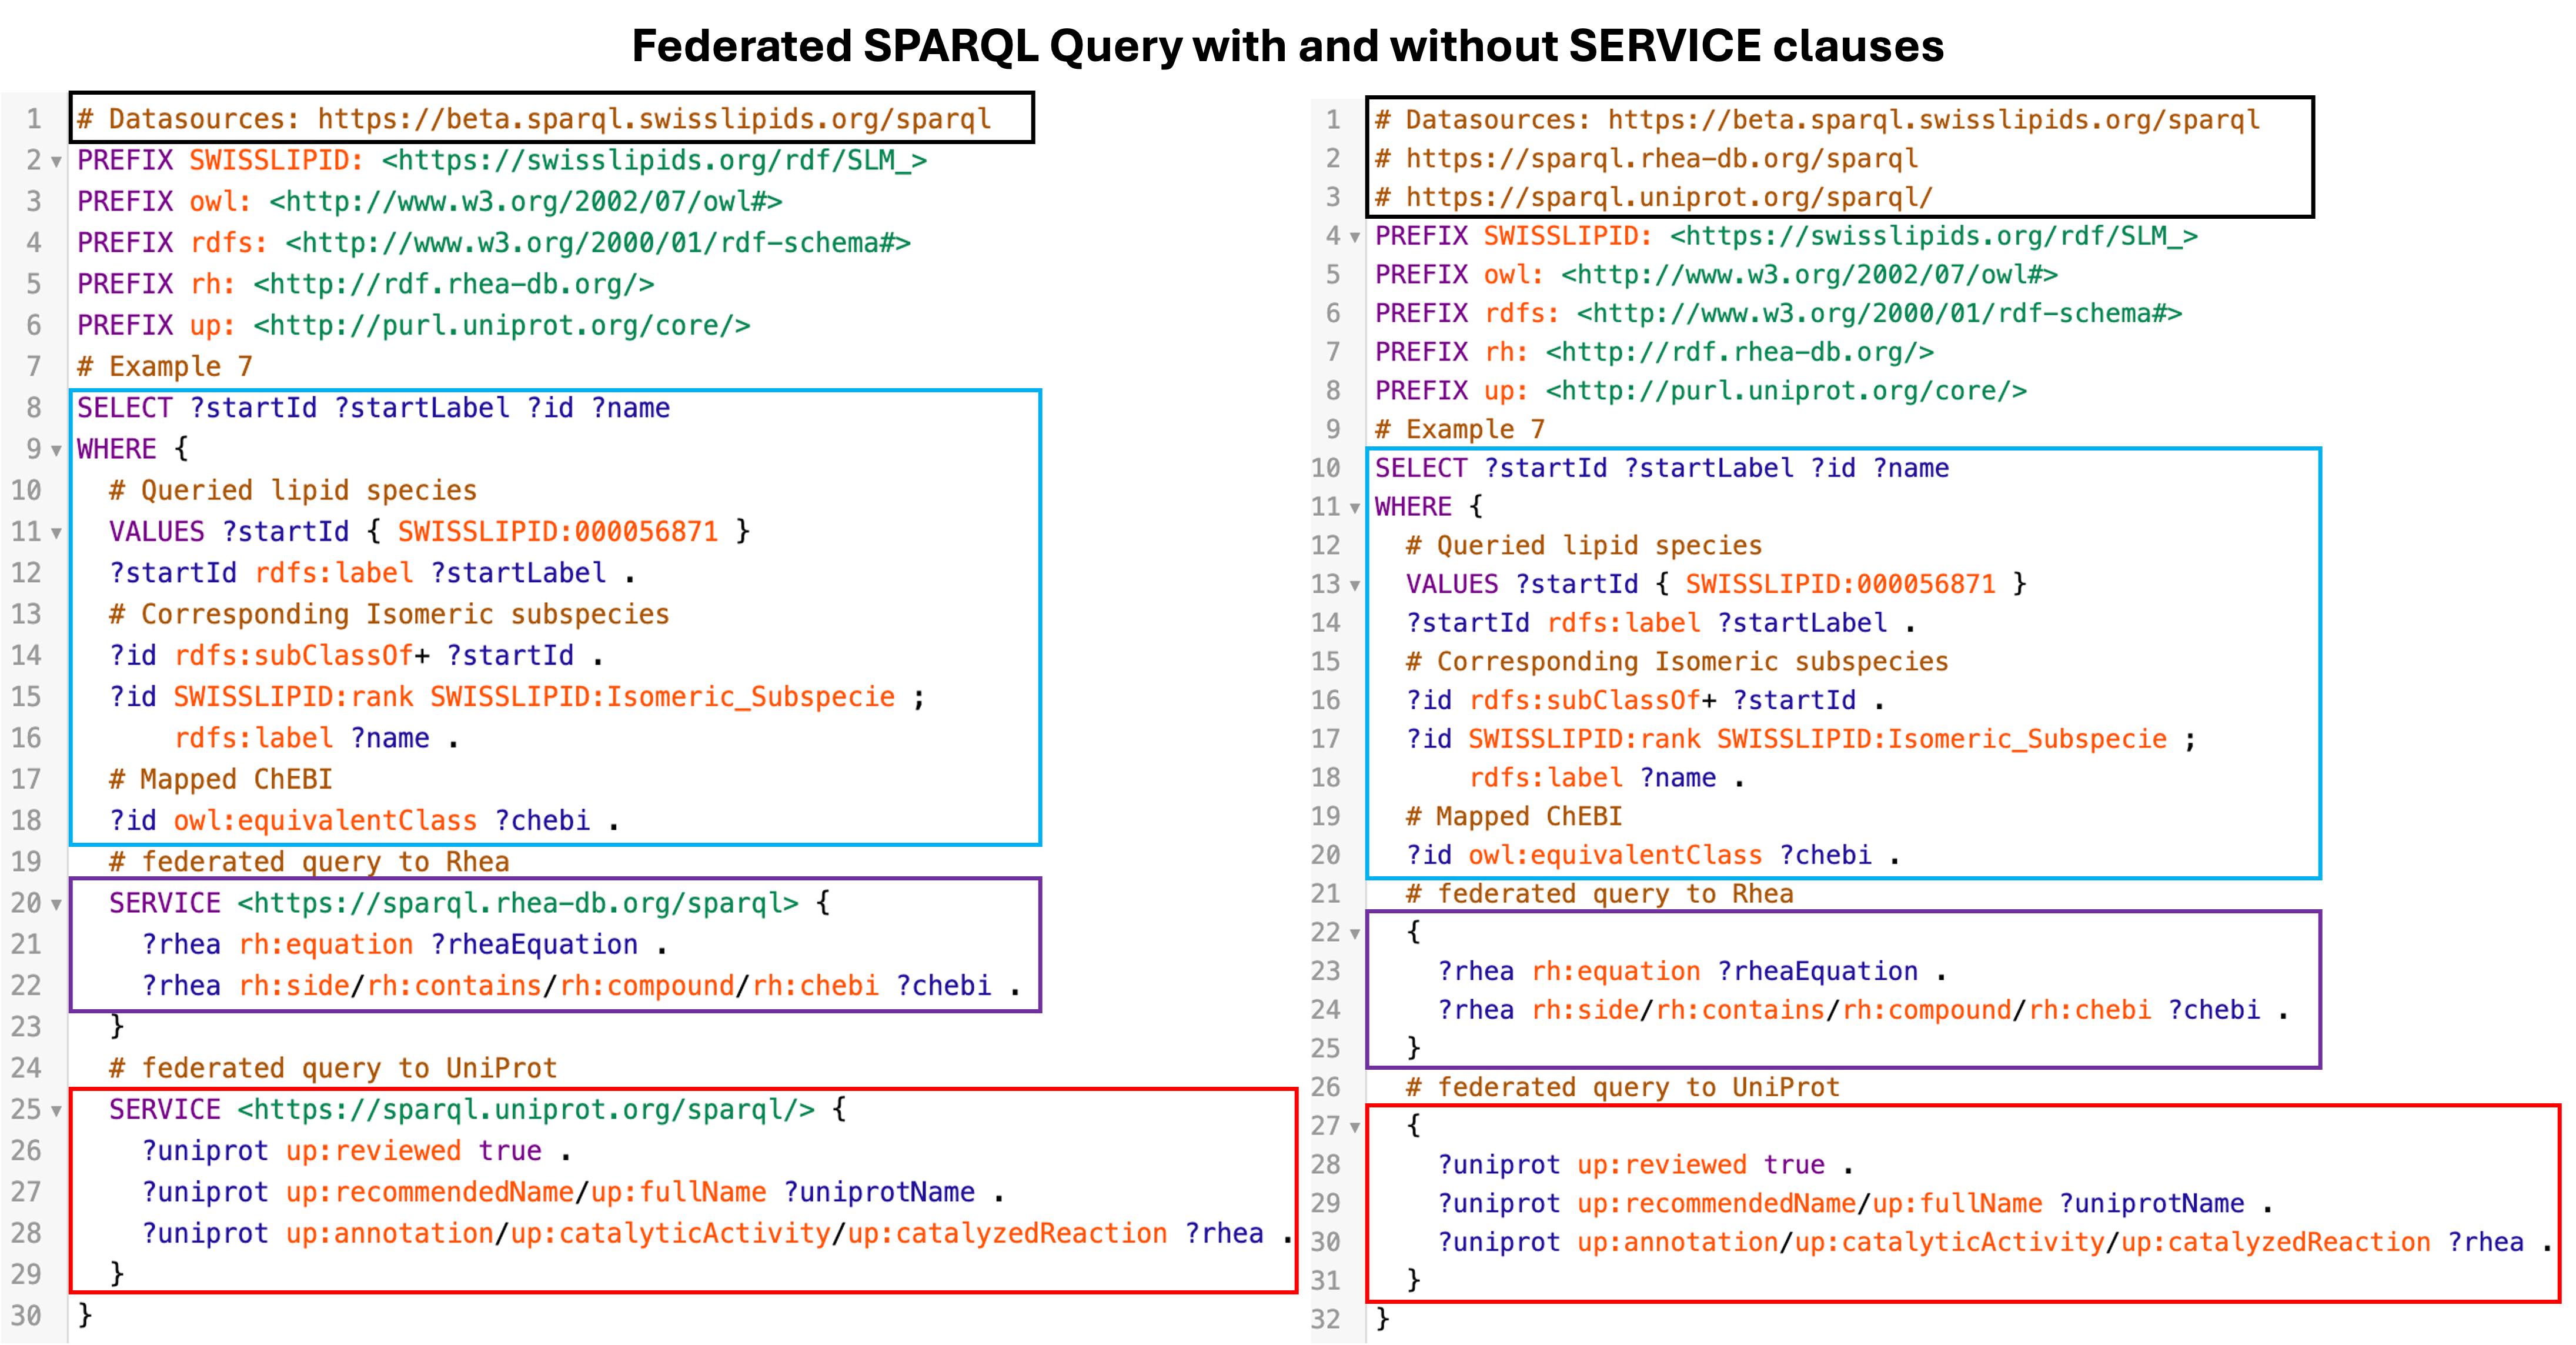
\includegraphics[width=1.0\textwidth]{query_content/sparql_query.png}
    \caption{
        Comparison of a federated SPARQL query manual server-side federation with \texttt{SERVICE} clauses (left) versus the equivalent query using client-side automated federation strategies without \texttt{SERVICE} clauses (right). Black box shows SPARQL endpoint URLs, Blue, Purple, and Red boxes designate sub-sections of the query sent to different endpoints.
    }
    \label{fig:sparqlQuery}
\end{figure}

\textbf{SPARQL} is the W3C-standard query language for retrieving and manipulating data stored in Resource Description Framework (RDF) format~\cite{Feigenbaum2013SPARQL}. 
\textbf{SPARQL federation} extends this model by enabling a single query to integrate the data of multiple, distributed data sources.
Figure~\ref{fig:sparqlQuery} displays two forms of a representative federated query (query \textit{7} in this study).

A crucial step in federated SPARQL query processing is \textit{source selection}: deciding which parts of a query are evaluated by which data sources. 
This can be specified \textit{manually} with the SPARQL 1.1 \texttt{SERVICE} keyword, as in the left panel of Figure~\ref{fig:sparqlQuery}, or handled \textit{automatically} by a client-side federation engine given only the query and target sources, as in the right panel. 
In both cases, \textit{query planning}, including join ordering, reducing intermediate results, and deciding whether joins are executed locally or at remote endpoints, also has a significant impact on overall query performance~\cite{Schmidt2010Foundations}. 
Automatic federation engines use different strategies for source selection, query partitioning, and optimization, and are further discussed in Section~\ref{sec3.1}.

The SPARQL query itself is a key factor in federated query performance. 
Even over a single endpoint, evaluation becomes more challenging as query structure grows in complexity and size.
In particular, the evaluation of basic graph patterns is known to be NP-complete, and the addition of operators such as \texttt{OPTIONAL} and \texttt{UNION} further increases evaluation complexity \cite{Perez2009Semantics}. 
Queries with many triple patterns can also produce large intermediate results and costly join operations, making planning and execution challenging~\cite{Schmidt2010Foundations}. 
In federated settings, these challenges are amplified: query engines must not only optimize joins and intermediate results locally, but also coordinate query decomposition, data transfer, and join execution across multiple remote endpoints with limited statistics and higher communication costs. 
Consequently, even moderately complex SPARQL queries can become substantially harder to execute efficiently across multiple endpoints.


\section{Related Work}\label{sec3}
% Prior work largely studies algorithmic behavior under controlled conditions
Prior work on federated SPARQL querying has advanced algorithms for source selection, query planning, and distributed join processing, but have typically been evaluated under controlled benchmark conditions. 
While traditional, controlled benchmark settings yielded important insights into algorithmic efficiency, they provides a limited view of how federation behaves against public endpoints under dynamic real-world conditions. 
This study therefore shifts the focus from stable benchmark environments to operational behavior in public settings.

\subsection{Federated Querying Algorithms}\label{sec3.1}
% SPARQL federation and common execution strategies
% FedX, SPLENDID, and source-selection/query-planning trade-offs
SPARQL federation has been studied primarily as a problem of \textit{source selection} and efficient intermediate-result processing. 
Systems such as \textsc{FedX} and \textsc{SPLENDID} illustrate two influential execution styles: \textsc{FedX} performs source selection dynamically at query time, avoiding reliance on precomputed source catalogs~\cite{schwarte2011fedx}, whereas \textsc{SPLENDID} uses standardized dataset metadata, in particular VoID descriptions~\cite{w3cvoid}, to guide source selection and planning~\cite{splendid2011}.
Other approaches target volatile environments, such as \textsc{ANAPSID}~\cite{anapsid2011}, or rely on custom statistics and metadata, including HiBISCuS~\cite{Saleem2014HiBISCuS}, CostFed~\cite{Saleem2018CostFed}, and FedUP~\cite{davat2024fedup}. 
From an endpoint maintainer’s perspective, however, publishing and maintaining such metadata is optional and often costly; consequently, endpoint-exposed metadata is often incomplete or unavailable in practice~\cite{Vandenbussche2017SPARQLES}. 
Federation is therefore commonly framed as query optimization under incomplete statistics and limited coordination between independently operated endpoints~\cite{montoya2017federation}. 
Given the real-world focus of our study, we evaluate only algorithms that do not depend on non-standard metadata for automated federation. Other relevant approaches such as \textsc{ANAPSID} was not included because no public implementation was available.

Recent systems have also made practical experimentation with federation strategies easier. 
In particular, \textsc{Comunica} provides a modular query engine in which source-selection methods, query planners, and join algorithms can be combined and compared~\cite{taelman2018comunica}. 
This modularity enables hybrid strategies, such as replacing \texttt{ASK}-based source selection, as used in \textsc{FedX}, with \texttt{COUNT}-based alternatives. 
Using a shared execution framework also reduces performance differences caused by implementation details, such as programming language, libraries, or threading models, allowing comparisons to focus more directly on the federation strategy itself.


\subsection{Federated Querying Benchmarks \& Evaluations}\label{sec3.2}
% Prior evaluations of SPARQL federation
% Public biological SPARQL endpoints as operational infrastructure
Benchmarks and empirical evaluations have played an important role in federated SPARQL research.
\textsc{FedBench} provides curated datasets and queries for comparing federation engines~\cite{Schmidt2011FedBench,Saleem2014FedBench}, while \textsc{LargeRDFBench} extends this approach to larger data volumes and more demanding federation scenarios~\cite{Saleem2018LargeRDFBench}. 
Other work has questioned how well curated or synthetic workloads capture the structure and difficulty of real query behavior, for example in Wikidata-oriented benchmarking~\cite{Hernandez2015Wikidata}.

Although valuable for controlled comparison, these benchmarks typically assume stable execution environments and abstract away from operational characteristics of public SPARQL services, such as endpoint timeouts, rate limits, transient HTTP failures, changing metadata, and fluctuating responsiveness.
In real-world conditions, public endpoints can vary substantially in availability, interoperability, and performance~\cite{Vandenbussche2017SPARQLES}, and these factors can directly affect federated query execution, sometimes causing partial or complete failure.

Rather than proposing a new federation algorithm or benchmark suite, here we study how federated biological queries behave longitudinally over widely used public endpoints using three different federation strategies (one server-side and two client-side).
Our work therefore complements prior algorithmic and benchmark-focused research by assessing the impact of real-world operational fragility, failure modes, and the gap between controlled benchmark assumptions and real-world use.


\section{Methods}\label{sec4}

\subsection{General Study Design}\label{sec4.1}
This study is a 13-month longitudinal evaluation of SPARQL query federation over public endpoints, focusing on the practical executability of real federated queries rather than controlled benchmark performance. 
Using the curated real-world query records described in Section~\ref{sec4.2}, we analyzed individual query executions within federation approach configuration--date experiments, enabling comparison across both federation approaches and changes in endpoint behavior over time. 
Because the evaluated strategies were implemented in \textsc{Comunica} rather than by directly invoking native \textsc{FedX} or \textsc{SPLENDID} binaries, we refer to them as \textit{metadata-free} (e.g., \textsc{FedX}) and \textit{metadata-guided} (e.g., \textsc{SPLENDID}) federation approaches throughout the study.
References to the companion results webpage are made throughout the paper as embedded links and direct to the same base webpage at the URL: \url{https://ecrum19.github.io/fed-survey-results/}.

\subsection{Real-World Queries}\label{sec4.2}
\textbf{Queries.}
The query corpus was obtained from users of SIB-hosted biological SPARQL endpoints~\cite{Bolleman2025sibqueries}. 
It contains 67 federated queries, all created by domain experts to answer real-world questions or test realistic scenarios. 
These queries were characterized in a structured CSV containing the original example query URL, natural-language description, target endpoint, federated endpoints, relevance/background notes, a ``toy'' flag, execution notes, similarity annotations, known problems, and aliases~\cite{fedSurveyResultsRepo}. 
The experimental repository stores the same corpus, with reduced metadata, in JSON format~\cite{fedSparqlSurveyExperimentsRepo}. 
More than half of the queries have a confirmed real-world application or address an open question, and around one quarter have produced results published in peer-reviewed papers.

To test client-side \textit{automatic} source selection, a preprocessing script~\cite{fedSparqlSurveyExperimentsRepo} generates two versions of each query: a \textsc{SERVICE} form, corresponding to the original query with one target source and explicit \texttt{SERVICE} clauses, and a \textsc{no-service} form, in which \texttt{SERVICE} clauses are removed and multiple source targets are provided separately. 
Figure~\ref{fig:sparqlQuery} shows an example of both forms. 
We refer to experiments using the former as \textit{\textsc{SERVICE} experiments} and those using the latter as \textit{\textsc{no-service} experiments}.

Finally, all 67 queries were manually executed through the target endpoints' web interfaces to establish positive-control result sets for each query, reported in the \textit{service-control-31-03-2025-endpoint} experiment~~\cite{fedSurveyResultsRepo}.

To characterize workload complexity, we extracted per-query features from the curated corpus, including triple-pattern counts, \texttt{OPTIONAL} and \texttt{UNION} usage, property paths, \texttt{DISTINCT}, \texttt{LIMIT}, and the number of federation members. 
Corpus-level summaries are available on the \href{https://ecrum19.github.io/fed-survey-results/}{companion results webpage}. 
Queries contain 14.90 triple patterns on average, ranging from 2 to 34, and involve an average of 2.24 federation members. 
About half use \texttt{DISTINCT} (mean 0.54), while \texttt{LIMIT} is less common (mean 0.18). 
Property paths appear frequently (mean 1.27), but recursive paths are less common (mean 0.49), suggesting that complex path recursion is concentrated in a subset of queries. 
Most queries contain no \texttt{OPTIONAL} or \texttt{UNION} clauses, with both averaging about 0.15 occurrences per query.
Figure~\ref{fig:complexityQuery}, available in a larger, interactive version on the \href{https://ecrum19.github.io/fed-survey-results/}{companion results webpage}, presents a per-query view of workload complexity by ordering queries by triple-pattern count and grouping them by the number of federation members.
Query features were extracted using a reproducible analysis script~\cite{queryAnalysisSibFederatedRepo}, and the full per-query feature table is available in the results repository~\cite{fedSurveyResultsRepo}.

Overall, the query set consists of moderately complex federated queries, typically spanning two or three sources, rather than simple joins over small fragments. 
At the same time, these queries are not dominated by advanced SPARQL features, suggesting that execution difficulty arises primarily from federation itself rather than from unusually complex query syntax.

\begin{figure}
    \centering
    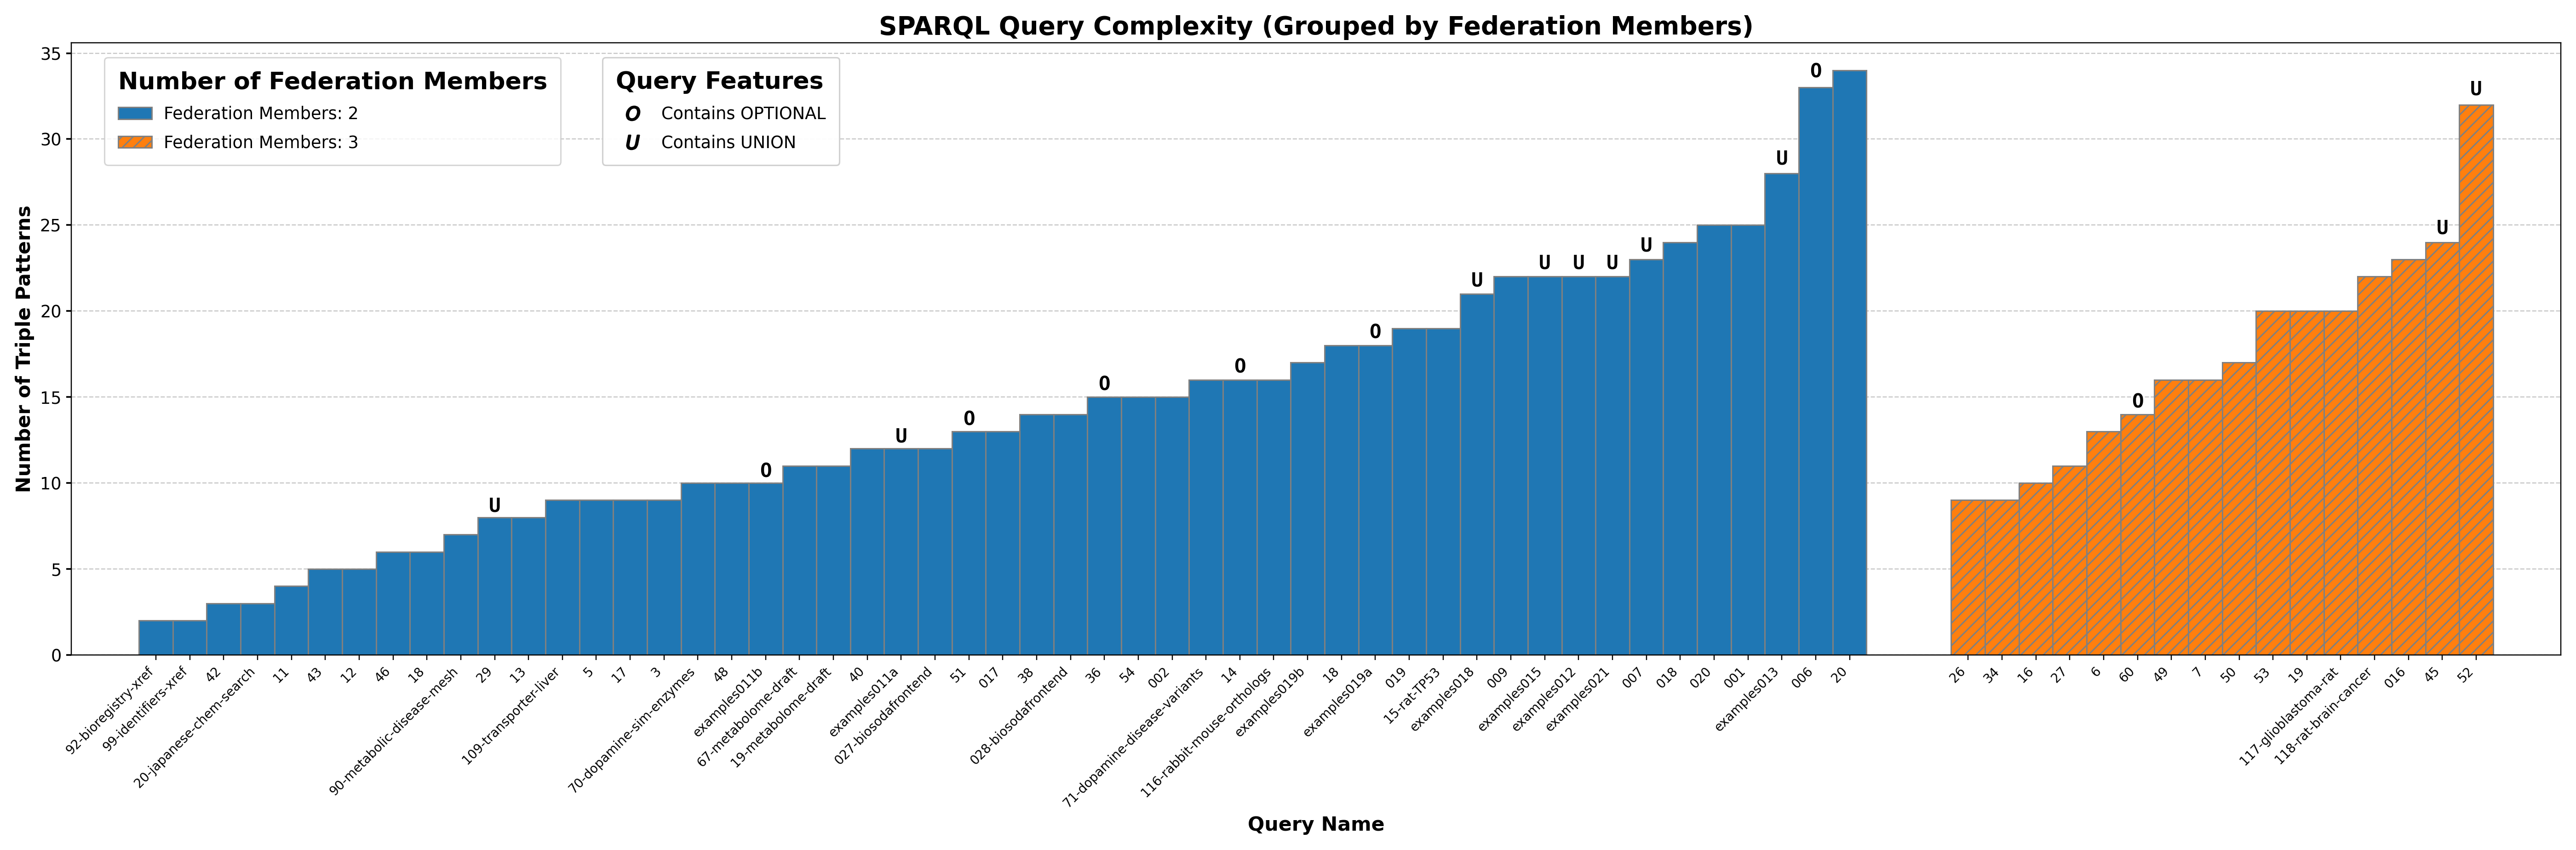
\includegraphics[width=1.0\textwidth]{query_content/Queries_Summary_Figure.png}
    \caption{
        Query complexity as a function of the number of triple patterns, federation members, and the presence of graph patterns. 
        More complex queries are those with OGPs, with a higher number of triple patterns and federation members, followed by those 
        with UGPs, following the same ordering in terms of triple patterns and federation members.
    }
    \label{fig:complexityQuery}
\end{figure}


Of the original 67 queries, 7 encountered errors early in experimentation and were excluded from \texttt{no-service} experiments.

% Preamble
\newcolumntype{Y}{>{\raggedright\arraybackslash}X}
\newcolumntype{L}[1]{>{\raggedright\arraybackslash}p{#1}}

\begin{table}[!t]
\centering
\scriptsize
\caption{SPARQL endpoints represented in the real-world query workload. 
Triple-Store was assessed through endpoint literature, server response, and endpoint service description data.
}
\label{tab:endpoints}

\setlength{\tabcolsep}{2pt}
\renewcommand{\arraystretch}{1.08}

\begin{tabularx}{\linewidth}{
    L{0.16\linewidth}
    Y
    L{0.22\linewidth}
    L{0.25\linewidth}
}
\hline
\textbf{Endpoint} 
& \textbf{Description} 
& \textbf{Triple-store} 
& \textbf{Endpoint URL} \\
\hline

UniProt~\cite{uniprot2025} 
& Protein sequence and functional annotations
& Virtuoso (past) / QLever (current)
& \tinyhref{https://sparql.uniprot.org/sparql}{sparql.uniprot.org/sparql} \\

Rhea~\cite{bansal2022rhea} 
& Biochemical and transport reactions
& Virtuoso
& \tinyhref{https://sparql.rhea-db.org/sparql}{sparql.rhea-db.org/sparql} \\

SwissLipids~\cite{Aimo2015SwissLipids} 
& Lipid structures
& unknown
& \tinyhref{https://beta.sparql.swisslipids.org/sparql}{beta.sparql.swisslipids.org/sparql} \\

Bgee~\cite{Bastian2025Bgee} 
& Gene expression for comparative analysis 
& Virtuoso
& \tinyhref{https://www.bgee.org/sparql}{bgee.org/sparql} \\

OrthoDB~\cite{Tegenfeldt2025OrthoDB} 
& Orthologous genes 
& Virtuoso
& \tinyhref{https://sparql.orthodb.org/sparql}{sparql.orthodb.org/sparql} \\

OMA~\cite{Altenhoff2024OMA} 
& Orthology and protein families 
& Virtuoso
& \tinyhref{https://sparql.omabrowser.org/sparql}{sparql.omabrowser.org/sparql} \\

biosoda~\cite{biosoda2021} 
& SPARQL federation server
& N/A
& \tinyhref{https://biosoda.unil.ch/emi/sparql}{biosoda.unil.ch/emi/sparql} \\

\hline

Wikidata~\cite{vrandecic2014wikidata} 
& General-purpose knowledge graph 
& Blazegraph
& \tinyhref{https://query.wikidata.org/sparql}{query.wikidata.org/sparql} \\

Wikidata--QLever 
& Alternative Wikidata endpoint 
& QLever
& \tinyhref{https://qlever.cs.uni-freiburg.de/api/wikidata}{qlever.cs.uni-freiburg.de/api/wikidata} \\

METRIN-KG~\cite{Tandon2026METRIN} 
& Plant metabolome and traits
& QLever
& \tinyhref{https://kg.earthmetabolome.org/metrin/api}{kg.earthmetabolome.org/metrin/api} \\

IDSM~\cite{Galgonek2021ChemWebRDF} 
& Small molecule database
& PostgreSQL
& \tinyhref{https://idsm.elixir-czech.cz/sparql}{idsm.elixir-czech.cz/sparql} \\

MBGD~\cite{Uchiyama2019MBGD} 
& Microbial genomes
& Virtuoso
& \tinyhref{http://sparql.nibb.ac.jp/sparql}{sparql.nibb.ac.jp/sparql} \\

STRING-DB~\cite{Szklarczyk2025STRING} 
& Functional protein association networks 
& Virtuoso
& \tinyhref{https://string-db.org/sparql}{string-db.org/sparql} \\

Allie~\cite{Yamamoto2011Allie} 
& Abbreviation and long-form searches 
& Virtuoso
& \tinyhref{http://data.allie.dbcls.jp/sparql}{data.allie.dbcls.jp/sparql} \\

EPO~\cite{Kracker2018} 
& Linked patent data
& unknown
& \tinyhref{https://data.epo.org/linked-data/query}{data.epo.org/linked-data/query} \\

EUNIS
& Biodiversity and species data
& unknown
& \tinyhref{https://semantic.eea.europa.eu/sparql}{semantic.eea.europa.eu/sparql} \\

data.europa.eu 
& European open data
& Virtuoso
& \tinyhref{https://data.europa.eu/sparql}{data.europa.eu/sparql} \\

GlyConnect~\cite{Alocci2019GlyConnect} 
& Glycoproteomics data 
& GraphDB
& \tinyhref{https://glyconnect.expasy.org/sparql}{glyconnect.expasy.org/sparql} \\

MeSH~\cite{bushman2015} 
& Medical Subject Headings (MeSH)
& unknown
& \tinyhref{https://id.nlm.nih.gov/mesh/sparql}{id.nlm.nih.gov/mesh/sparql} \\

Bioregistry~\cite{Hoyt2022Bioregistry} 
& Registry of biomedical identifiers 
& RDFLib endpoint
& \tinyhref{https://bioregistry.io/sparql}{bioregistry.io/sparql} \\

Identifiers.org~\cite{Juty2012Identifiers} 
& Persistent identifier registry 
& unknown
& \tinyhref{https://sparql.api.identifiers.org/sparql}{sparql.api.identifiers.org/sparql} \\

\hline
\end{tabularx}
\end{table}

\textbf{Endpoints.}
All SPARQL endpoints used in this study are listed in Table~\ref{tab:endpoints}. 
Endpoints above the horizontal line are \textit{target endpoints}, to which complete queries are submitted in \textsc{SERVICE} experiments. 
For queries with explicit \texttt{SERVICE} clauses, these targets initiate remote requests during execution. 
Endpoints below the line are \textit{federates-with endpoints}: they appear in \texttt{SERVICE} clauses and are queried remotely, but are not direct submission targets. 
This distinction therefore separates endpoints acting as server-side federation engines (\textit{target endpoints}) from those acting as remote federated data sources (\textit{federates-with endpoints}).

Table~\ref{tab:endpoints} also reports the underlying triple-store for target endpoints. 
A \textit{triple-store} is an RDF database optimized for SPARQL query evaluation, with systems differing in indexing, planning, federation support, and scalability~\cite{Erling2009VirtuosoRDF,bast2017qlever}. 
For UniProt, we distinguish the Virtuoso-based deployment used before May 2025 from the QLever deployment introduced in a May 2025 migration. 
Triple-stores for other endpoints were identified from literature, service descriptions, or HTTP response headers (\texttt{Server}, \texttt{X-Powered-By}, \texttt{Via}, and/or \texttt{Link}) obtained with \texttt{curl} requests; endpoints whose backend could not be determined are marked as ``unknown''.

Several endpoint-specific notes apply. 
METRIN-KG is used as the current production endpoint for queries that previously referred to DBGI, reflecting that resource's migration to a QLever-backed deployment. 
neXtProt~\cite{ZahnZabal2020neXtProt} was excluded because it has not been publicly hosted or maintained since Fall 2023. 


\subsection{Federation Approaches}\label{sec4.3}
The \textsc{Comunica} query engine framework~\cite{taelman2018comunica} v4.3.0 was used for both server-side manual federation (\textsc{SERVICE} experiments) and client-side automated federation (\textsc{no-service} experiments), while keeping the client-side execution environment constant. 
In \textsc{SERVICE} experiments, \textsc{Comunica} acts only as an external client: the complete query, including its explicit \texttt{SERVICE} clauses, is submitted to a single target endpoint, which is then responsible for federation tasks, carrying out remote requests, intermediate result joins, and returning the final results.
In contrast, in \textsc{no-service} experiments, with \texttt{SERVICE} clauses removed and multiple sources provided, \textsc{Comunica} performs client-side automated federation according to the predefined configuration.
Thus, the same engine is used in both settings, but automated federation is only performed in \textsc{no-service} experiments.

\begin{table}[t]
    \centering
    \scriptsize
    \caption{
        Comunica federation configurations used in our server-side automated federation experiments.
        A checkmark indicates the presence, while a dash indicates the absence of an approach within a configuration.
        \texttt{-NRL} variants disable client-side request rate limiting while leaving other configuration choices unchanged.
    }
    \label{tab:comunicaConfigs}

    \setlength{\tabcolsep}{3pt}
    \renewcommand{\arraystretch}{1.08}

    \begin{tabularx}{\linewidth}{Xccccc}
        \hline
        \textbf{Configuration}
            & \textbf{ASK}
            & \textbf{COUNT}
            & \textbf{VoID}
            & \textbf{Large est.}
            & \textbf{Rate limit} \\
        \hline

        \texttt{NOMETA-ASK}        & \checkmark & --         & --         & --         & \checkmark \\
        \texttt{NOMETA-COUNT}      & --         & \checkmark & --         & --         & \checkmark \\
        \texttt{VOID-TRIPLE}       & \checkmark & --         & \checkmark & --         & \checkmark \\
        \texttt{VOID-BLOCK}        & \checkmark & --         & \checkmark & \checkmark & \checkmark \\
        \texttt{-NRL}              & --         & --         & --         & --         & -- \\

        \hline
    \end{tabularx}
\end{table}

For client-side automated federation, defined configuration guide query processing.
Table~\ref{tab:comunicaConfigs} represents the comunica configs chosen to isolate the main client-side automated federation approaches, especially for source-selection and query planning, evaluated in this study.
Operationally, metadata-free configurations identify relevant sources at runtime using lightweight endpoint probes such as \texttt{ASK} or \texttt{COUNT} queries, and group compatible operations for remote delegation when possible~\cite{schwarte2011fedx}. 
Separating \texttt{ASK} vs. \texttt{COUNT} additionally allowed us to compare lightweight source pruning (\texttt{ASK}) against more expensive cardinality estimation (\texttt{COUNT}).
Metadata-guided configurations instead use available VoID descriptions and pre-computed dataset statistics for source selection and cardinality estimation, reducing runtime probing when such metadata are available~\cite{splendid2011,w3cvoid,hagedorn2014resource}. 
Thus, the configurations vary in their reliance on pre-existing endpoint metadata versus live endpoint interaction.
Because experiments were run against public endpoints rather than controlled benchmark servers, \textsc{Comunica} was configured with pragmatic rate-limiting safeguards to reduce the impact of server-side rate limits~\cite{rfc9110}. 

These configurations were chosen to isolate the main source-selection and planning assumptions evaluated in this study.
The \textsc{NOMETA-ASK} and \textsc{NOMETA-COUNT} settings represent index-free strategies that rely on live endpoint probing, allowing us to compare lightweight source pruning against more expensive cardinality estimation.
The \textsc{VOID-TRIPLE} and \textsc{VOID-BLOCK} settings represent index-assisted strategies that use available VoID metadata, allowing us to evaluate whether endpoint-provided statistics improve planning at either the triple-pattern (\textsc{VOID-TRIPLE}) or larger query-block (\textsc{VOID-BLOCK}) level.
Together, these four configurations cover the principal trade-off between runtime probing and metadata-assisted planning, while the \texttt{-NRL} variants separately test the effect of client-side rate limiting without changing the underlying federation strategy.

All configurations were applied to the experimental \textsc{Comunica} engine using a \href{https://github.com/ecrum19/fed-sparql-survey-expts/blob/main/comunica_configuration.py}{configuration script}.


\subsection{Experimental Set-up}\label{sec4.4}

\textbf{Observation period.}
The testing campaign comprised 20 experiments conducted between March 2025 and April 2026. 
We therefore treat the study as longitudinal, with repeated executions of the same workload and configuration families at multiple time points.

\textbf{Execution environment.}
Experiments ran on an Ubuntu 24.04.1 virtual machine with an Intel Core i5-9500 CPU (6 cores, 3.0 GHz), 64 GB RAM, a 468 GB NVMe SSD, and Linux kernel 6.8.0-45-generic. 
All queries targeted public endpoints, not local mirrors or replicated stores.

\textbf{\textsc{SERVICE} experiment workflow.}
In \textsc{SERVICE} experiments, queries were executed in their original form, preserving explicit \texttt{SERVICE} clauses and submitting the complete query to a single target endpoint. 
Each query was submitted with a single target endpoint as datasource while retaining its embedded \texttt{SERVICE} clauses; therefore, \textsc{Comunica} performed no clinet-side automatic federation strategies. 

\textbf{\textsc{no-service} experiment workflow.}
The reproducible \textsc{no-service} workflow, documented in the study's experimental repository~\cite{fedSparqlSurveyExperimentsRepo}, follows four steps:
(1)\textsc{\seqsplit{query\_sort.py}}, (2)\textsc{\seqsplit{comunica\_configuration.py}}, 
(3)\textsc{\seqsplit{comunica\_run.py}}, and (4)\textsc{\seqsplit{localize\_results.sh}} \& \textsc{\seqsplit{organize\_data.py}}.
These correspond to query preparation, configuration selection, execution, and post-processing/summary generation, respectively. 
During execution, \texttt{\seqsplit{comunica\_run.py}} initializes a fresh \textsc{Comunica} engine instance via \texttt{\seqsplit{query-dynamic.js}} for each query executed. 
Datasources are read from the query header, SPARQL-JSON\cite{sparql11resultsjson} is requested as output, debug logging is enabled, and standard error is written to a per-query log file from which experiment-level summaries are generated. 

\textbf{Timeouts and retries.}
The execution script does not impose a wrapper-level wall-clock timeout but we do record wall-clock runtime from the logged start and end timestamps. 
Query termination is therefore determined by completion, endpoint-side failure, engine-level failure, or external process termination and timeout-like phenomena are captured indirectly through these measured timestamps and failure modes. 
To reduce rate-limit effects, the execution script uses \texttt{--httpRetryCount=50} and inserts a one-second pause between queries if an HTTP-429 error~\cite{Nottingham2012RFC6585} is encountered.

\textbf{Endpoint request burden and error types.}
During experiments, we tracked the number of HTTP requests per query and the final error text or category when execution failed. 
These data support three operational metrics: endpoint request burden, endpoint-associated error rate, and failure-type distribution. 
In a longitudinal public-endpoint setting, these metrics help distinguish whether execution changes stem from client-side federation planning, network or endpoint instability, or endpoint-side request handling.

\textbf{Definition of success and failure.}
An execution is considered to have \emph{produced results} if it returns parseable output conforming to the SPARQL 1.1 Query Results JSON Format~\cite{sparql11resultsjson}. 
Empty and non-empty result sets are distinguished using \texttt{results\_count}. 
Executions that produce no parseable output or terminate through an exception/error path are treated as explicit failures.
For the remainder of the study, we define \emph{execution success rate} as the proportion of executions that have produced a non-empty result set (i.e. results\_count > 0). 

\textbf{Result Correctness.}
This study does not provide a ground-truth assessment of the semantic correctness of returned SPARQL bindings.
In public federated SPARQL settings, establishing true correctness would require centralizing all relevant data from every participating endpoint and evaluating each query over a complete reference dataset, which was infeasible due to data scale, infrastructure requirements, and hardware constraints.
Consequently, we use \textit{result-set size agreement} as a proxy for correctness rather than claiming to verify individual bindings.

For each query, the reference result-set size was defined as the maximum result count observed under manual \textsc{SERVICE} execution, where the query retained its explicit \texttt{SERVICE} clauses and was evaluated against the single provided target endpoint.
Subsequent executions were considered consistent with this proxy when they produced the same result count as the reference value.
Thus, throughout this study, ``correctness'' refers only to agreement in result-set size, not to equality of returned bindings or semantic completeness.

\textbf{Temporal reproducibility.}
To assess reproducibility over time, identical query--configuration pairs are compared across dated runs. 
At minimum, reproducibility can be operationalized at three levels: whether the execution remained successful, whether it continued to return a non-empty result, and whether its error mode changed across time. 
This metric is central to the present study because the same query may be executable at one time point and non-executable at another, even under an unchanged engine configuration.


\section{Results}\label{sec5}
% Ground-truth control SERVICE experiments
We first compared the March 2025 \textsc{SERVICE} experiments to assess whether Comunica introduced systematic differences relative to direct endpoint execution.
Manual endpoint execution performed slightly better than the Comunica-mediated control, with higher \emph{execution success rates} (\(65.2\%\) vs. \(60.6\%\)) and fewer explicit errors (\(30.3\%\) vs. \(34.8\%\)).
However, the close agreement suggests that Comunica did not introduce a major confounding effect in subsequent experiments.

\begin{figure*}[t]
    \centering

    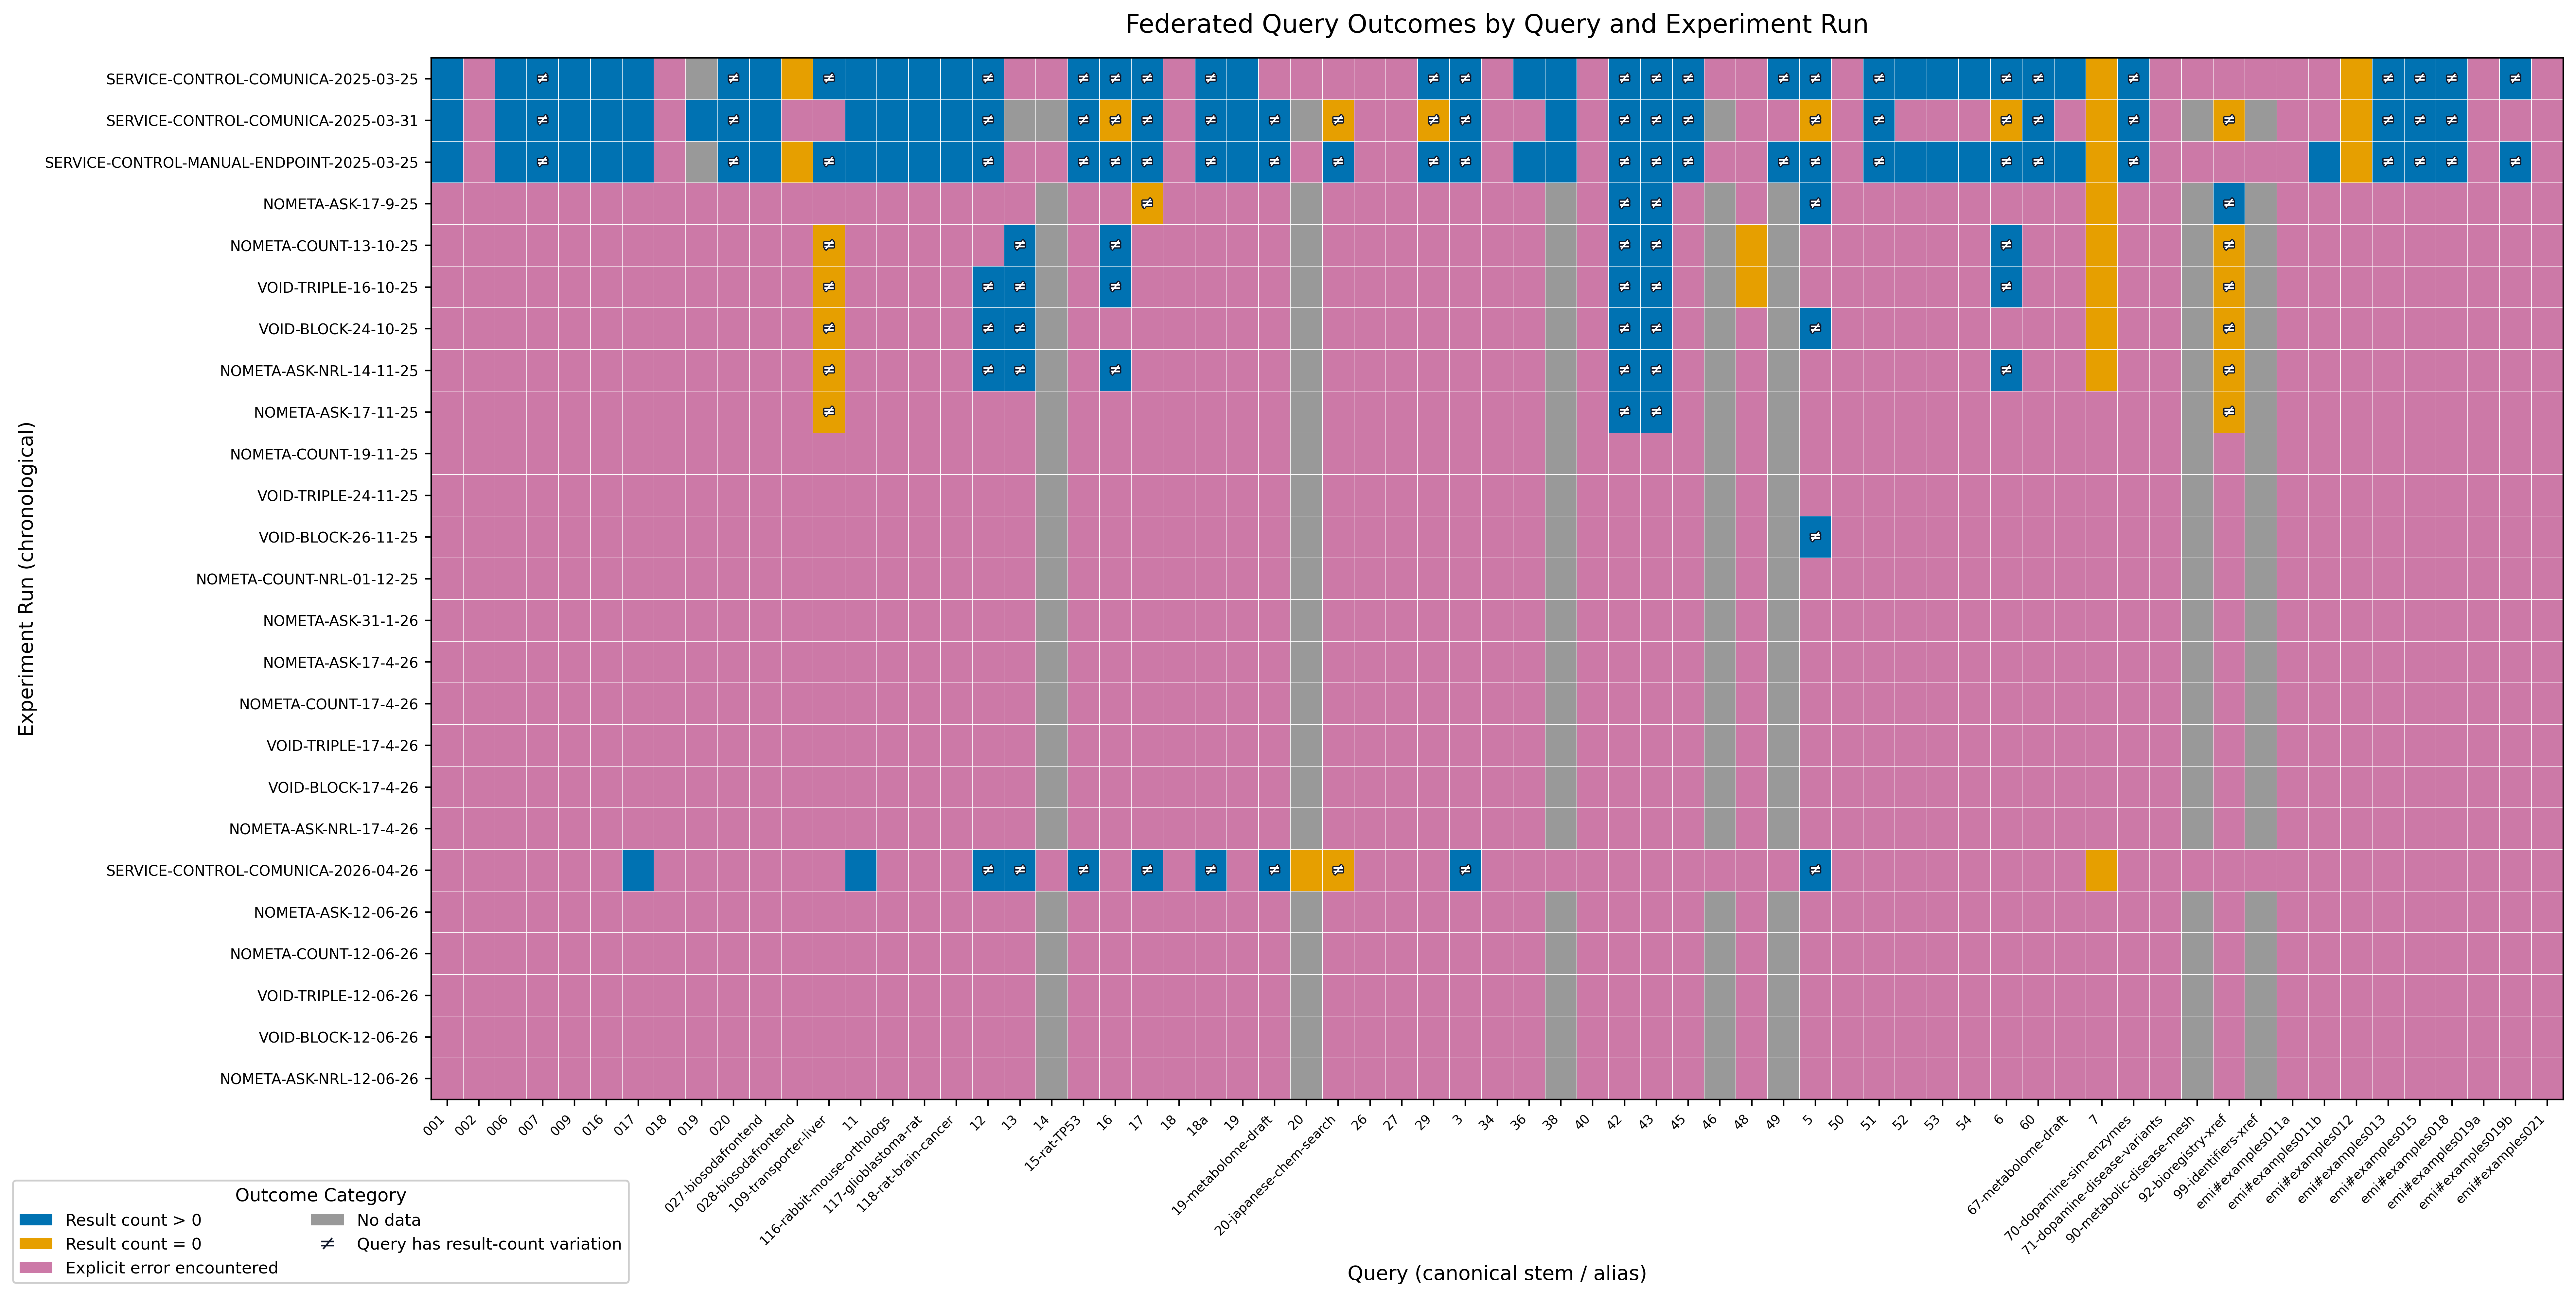
\includegraphics[width=\textwidth]{Results/heatmap.png}

    \caption{
        Overview of federated query experiment outcomes across 25 experiment runs of the 67-query test set.
        Outcome matrix cells represent whether a query produced a non-empty result set (blue), an empty result set (yellow), an explicit error (pink), or data was missing for that run (gray).
        The heatmap shows that failures are widespread across the workload.
        For an interactive, expandable version of this figure see the \href{https://ecrum19.github.io/fed-survey-results/?mode=query&query=001&queryVariant=original}{results repository webpage}.
    }
    \label{fig:allQueries}
\end{figure*}
% General findings
Figure~\ref{fig:allQueries} shows all experimental query executions chronologically, with older experiments at the top.
A larger interactive version is available in the \textit{Overview Figures} section of the \href{https://ecrum19.github.io/fed-survey-results/}{results webpage}.
Overall, \textsc{SERVICE} experiments performed far better than \textsc{no-service} client-side automated federation experiments: \textsc{SERVICE} experiments had \emph{execution success rate} of \(47.3\%\), and a \(46.2\%\) explicit error rate.
In contrast, \textsc{no-service} experiments had only a \(3.0\%\) \emph{execution success rate}, and \(95.1\%\) failed with explicit errors.
Thus, removing explicit \texttt{SERVICE} clauses and relying on automatic client-side federation reduced successful result production by roughly an order of magnitude and nearly doubled the error rate.
\textsc{no-service} experiments were also slower and more variable, with a median runtime of 4.47 seconds and a 90th percentile of 247.92 seconds, suggesting many failures involved severe slowdowns or stalled execution.


\subsection{Temporal Degradation of Query Success}\label{sec5.1}
% Discussion about decrease in efficacy over time ...
\begin{figure*}[t]
    \centering

    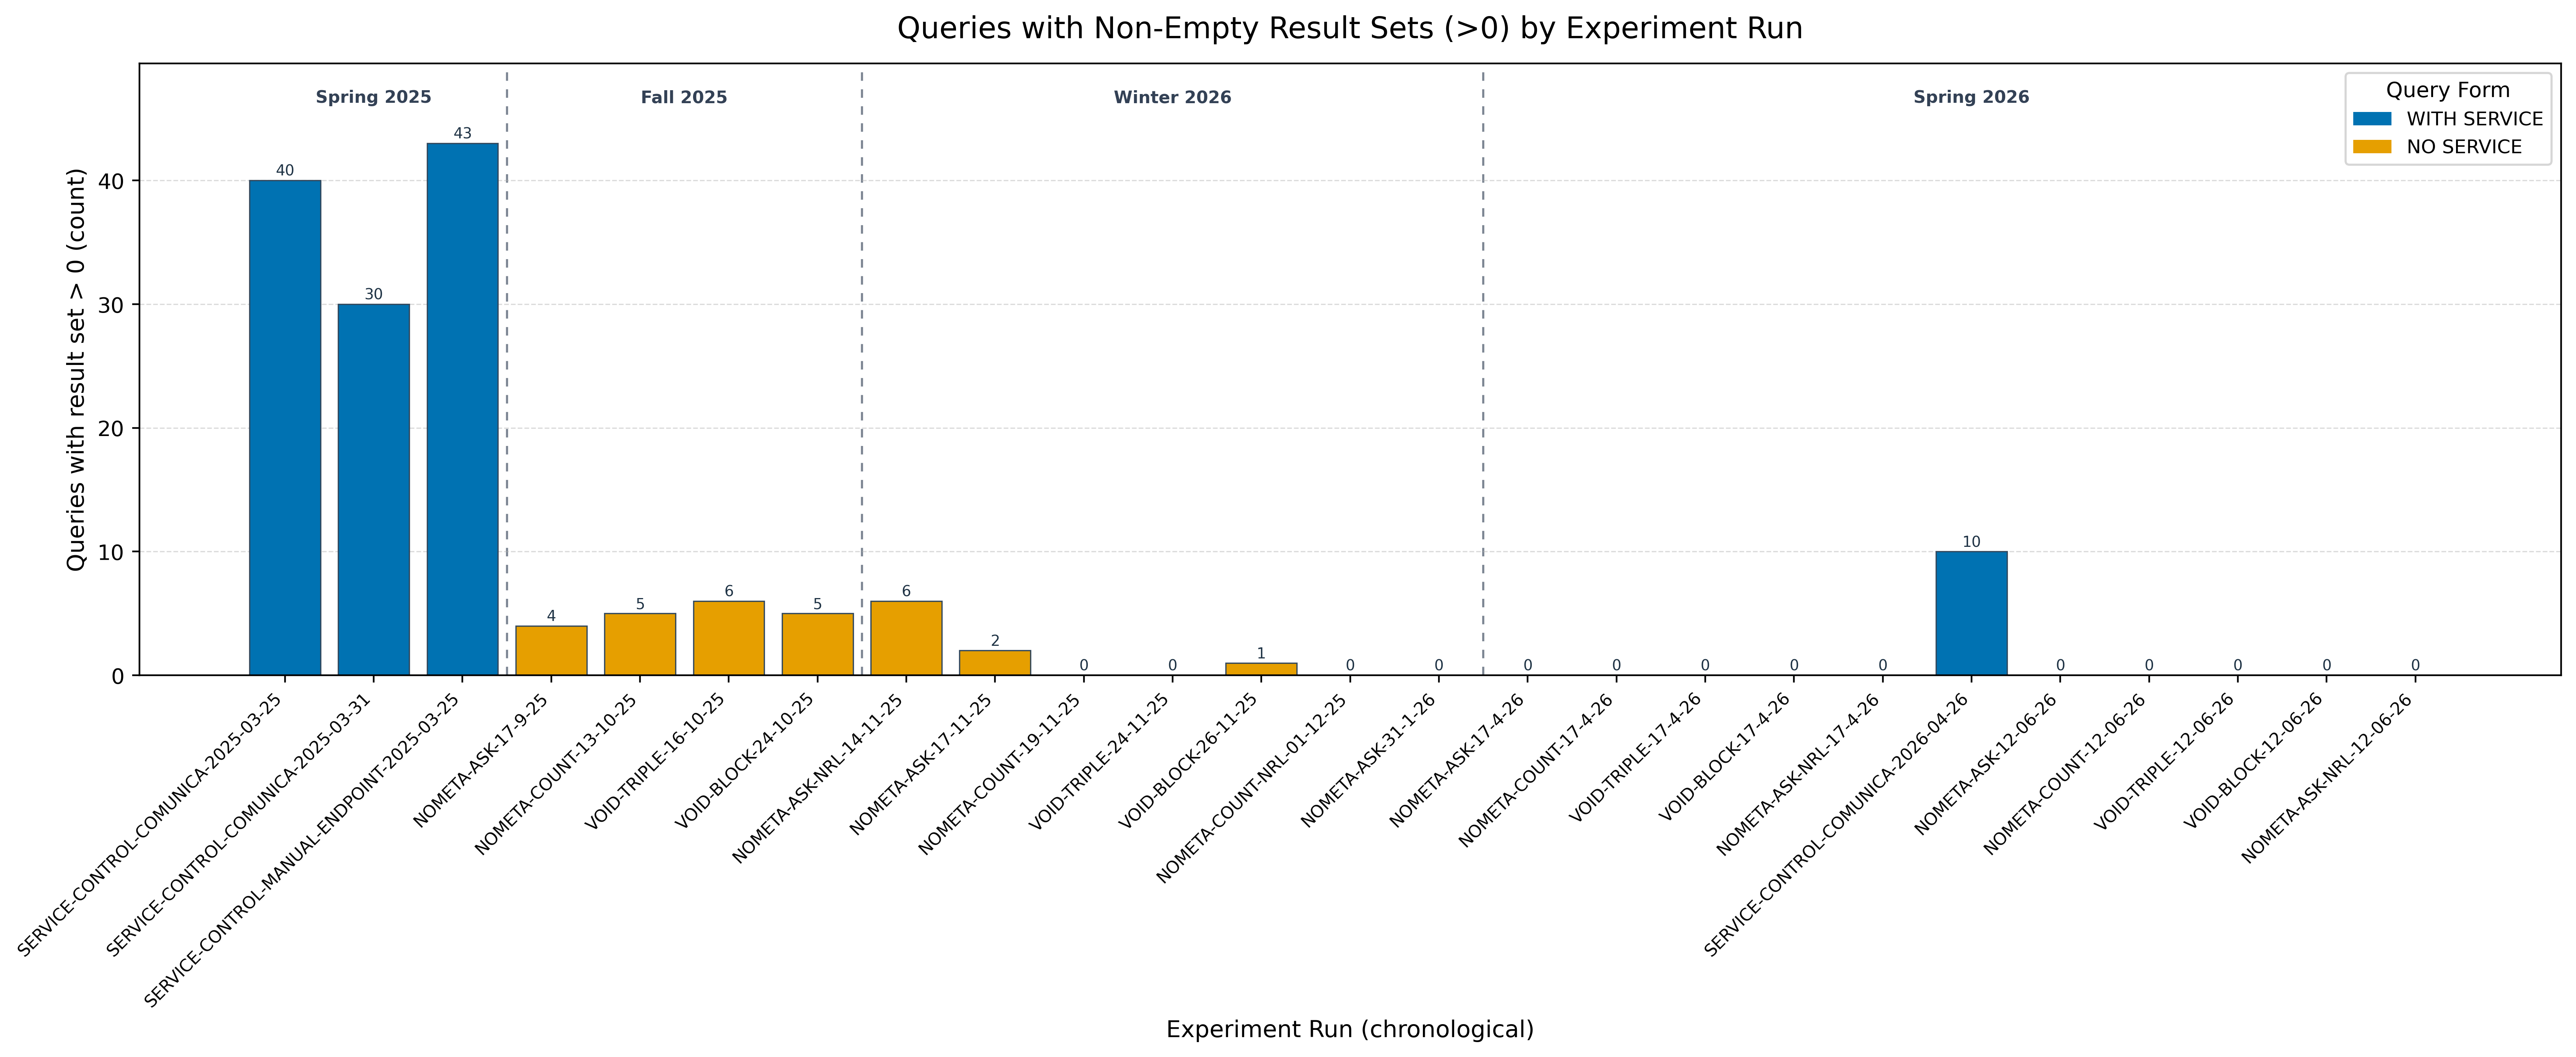
\includegraphics[width=\textwidth]{Results/trend.png}

    \caption{
        The trend showing a decrease in the number of queries producing non-empty result sets in each run, grouped by experiment form.
        Explicit \texttt{SERVICE} control runs produced substantially more non-empty result sets than \texttt{no-service} runs, while later runs show a marked decline in successful result production.
    }
    \label{fig:queriesTrend}
\end{figure*}

Figure~\ref{fig:queriesTrend} illustrates the degradation of federated query success chronologically, showing that more queries obtained results in chronologically earlier executions for both \textsc{SERVICE} and \textsc{no-service} experiments.
For ease of comparison, we separated experimental executions into 4 distinct chronological groups: Spring 2025, Fall 2025, Winter 2026, and Spring 2026.
An in-depth, interactive data display of these time-based partitions can be viewed in the \textit{Monthly Views} section of the \href{https://ecrum19.github.io/fed-survey-results/}{results webpage}.

During Spring 2025, which included only \textsc{SERVICE} experiments, performance was strongest, with \(58.5\%\) execution success and \(34.2\%\) explicit errors.
By Fall 2025, execution success dropped to \(8.5\%\), explicit errors rose to \(85.9\%\), and runtimes became highly heavy-tailed, with the 90th percentile reaching approximately \(1.07\times 10^4\) seconds and high HTTP request burden.
Winter and Spring 2026 remained low-success, high-error phases, with execution success rates of \(2.1\%\) and \(2.7\%\), and error rates of \(96.7\%\) and \(96.5\%\), respectively.
Notably, the Spring 2026 \textsc{SERVICE} experiments also performed far worse than Spring 2025, with only \(14.9\%\) execution success.
Although extreme runtime tails decreased by Spring 2026, successful result production did not recover.
Overall, Figure~\ref{fig:queriesTrend} shows this clear temporal decline in queries producing results.

Beginning in Fall 2025, many previously successful queries began failing after only 3--6 HTTP requests and roughly 4 seconds. 
Per-query logs show repeated \texttt{Server reported client-side error} events for \url{https://sparql.uniprot.org/sparql/}, with HTTP \texttt{403 Forbidden} errors, including for formerly stable queries such as \texttt{42}, \texttt{12}, and \texttt{16}. 
This indicates that server-side restrictions became a major contributor to the observed drop in success. 
According to the primary UniProt server administrator, this period coincided with increased LLM crawler traffic, including crawlers that ignored \texttt{robots.txt} guidelines.

Even when queries produced results, outputs were often unstable across repeated runs. 
Overall, 68.7\% of queries returned varying result counts, and 24 queries produced three or more distinct result-count outcomes, marked by the \texttt{"$\neq$"} icon in Figure~\ref{fig:allQueries}. 
For example, \texttt{92\_uniprot\_bioregistry\_iri\_translation} returned 194 results in Fall 2025, later returned parseable but empty outputs, and eventually failed in Winter 2026. 
Thus, live federation can degrade not only through hard failures, but also through empty or otherwise reduced result sets.

\subsection{Explicit Error Taxonomy}\label{sec5.2}
% discuss the explicit errors observed and point to website for more details
Across experiments, failures clustered into a small set of recurring categories, interactively visualized in the \textit{Query error-type heatmap by experiment run} on the \href{https://ecrum19.github.io/fed-survey-results/?mode=query&query=001&queryVariant=original}{results webpage}. 
The most frequent were \textsc{client-side HTTP} errors (n=577), followed by \textsc{server-side HTTP} errors (n=222), \textsc{transport-level} failures (n=85), \textsc{other} errors (n=80), and \textsc{timeout-related} errors (n=63). 
\textsc{Client-side HTTP} errors correspond to 4xx endpoint rejections or invalid-request responses, while \textsc{server-side HTTP} errors correspond to 5xx responses after request acceptance. 
\textsc{Timeout-related} errors include explicit endpoint limits and long-running requests that could not remain open long enough to complete. 
We classify \texttt{fetch failed} as \textsc{transport-level}, since no complete parseable response was received, even though some cases may reflect timeout-like connection aborts. 
\textsc{Other} errors include unexpected responses, such as HTTP 200 replies containing HTML error pages instead of valid SPARQL results (e.g., by endpoints deployed with a Virtuoso triple-store).

These failures reflect both endpoint-side constraints and erroneous client-side federation behavior. 
Endpoint-related failures included HTTP 403 rejections, server errors, aborted response bodies, malformed responses, and timeout-like interruptions. 
Client-side failures occurred when federation plans generated very large intermediate joins or excessive request volumes, sometimes exhausting resources with errors such as \texttt{Reached heap limit}. 
In extreme cases, individual queries issued hundreds of thousands to millions of HTTP requests before failing or narrowly completing, indicating request-explosion behavior from poor automatic client-side federation plans. 
Examples include query \texttt{6} with 924{,}299 requests, query \texttt{13} with 742{,}417 requests, and query \texttt{16} with 553{,}202 requests in experiment \texttt{NOINDEX-ASK-17-9-25}.


\subsection{HTTP Requests and Queries that Obtain Results}\label{sec5.3}
% Talk about HTTP requests and outcome trends --> point to big HTTP request table
We examined whether successful \textsc{no-service} executions differed from failures in HTTP request burden, restricting the analysis to runs with valid request counts ($n=954$). 
Because request counts were highly skewed, we report both means and medians, and use permutation tests and Mann--Whitney U tests as assumption-light complements to correlation estimates~\cite{altman1994quartiles,good2005permutation,mann1947test}.

Under a broad success definition, any execution without an explicit error, successful runs issued more requests than failures on average (46{,}366 vs. 16{,}663) and by median (22 vs. 6). 
However, the association was weak ($r=0.049$), with only marginal permutation-test support ($p=0.065$ for correlation; $p=0.064$ for mean difference).
Using a stricter definition of success as a non-empty result set, successful executions again showed higher request burden, both in mean (68{,}085 vs. 16{,}560) and median (580 vs. 6). 
The effect remained small ($r=0.068$), but was statistically supported by permutation tests ($p=0.036$ for correlation; $p=0.033$ for mean difference) and by a Mann--Whitney U test ($p<10^{-6}$).

Overall, successful client-side automatic federation was not associated with fewer endpoint interactions. 
Non-empty results often required more HTTP activity, likely due to source probing, remote subquery execution, and intermediate-result transfer. 
However, small effect sizes and large mean--median gaps show that request burden was highly uneven and dominated by outliers, making HTTP request count alone a weak predictor of success. 
Query- and experiment-specific plots are available in the \textit{Data Explorer} section of the \href{https://ecrum19.github.io/fed-survey-results/}{results webpage}.


\subsection{Comparison across federation approaches}\label{sec5.4}
Across the \textsc{no-service} experiments, all client-side automated federation algorithm families failed in most executions, with \emph{execution success rates} between only \(2.08\%\) and \(3.45\%\).
The corresponding counts were \(12/360\) for \textsc{NOMETA-ASK}, \(5/240\) for \textsc{NOMETA-COUNT}, \(6/180\) for \textsc{VOID-TRIPLE}, and \(6/174\) for \textsc{VOID-BLOCK}.
These results are visualized in the \textit{\textsc{no-service} algorithm efficacy comparison} on the \href{https://ecrum19.github.io/fed-survey-results/}{results webpage}.

Thus, all algorithms succeeded in a small minority of cases, but none was broadly robust for the tested workload. 
Differences between methods were modest: \texttt{VOID-TRIPLE} had the highest explicit-error-free rate, \texttt{VOID-BLOCK} the highest \emph{execution success rate}, and \texttt{NOMETA-COUNT} was consistently weakest. 
Success also varied substantially across runs, including some with \(0\%\) success, indicating general instability over time. 
Overall, VoID-based metadata-guided strategies provided only a small advantage over metadata-free strategies in \textsc{no-service} experiments.

The \texttt{-NRL} runs show that client-side rate-limit mitigation did not seem to impact \emph{execution success rates}. 
Similar success ratios are observed for queries completed in Fall 2025 with and without rate-limit mitigation, and by Spring 2026 all configurations converged to complete failure. 
This suggests that client-side naive throttling or backoff cannot overcome tighter server-side policies.


\subsection{Unique Study Challenges and Endpoint Instability}\label{sec5.4}

A number of later failures were caused by endpoint address changes outside the experiment’s control. 
Queries involving the former DBGI/EMI endpoint (14/67 queries) were affected by its migration to the production METRIN-KG endpoint at \url{https://qlever.earthmetabolome.org/api/metrin-kg}. 
Similarly, \url{https://biosoda.unil.ch/emi/sparql}, a temporary federation server targeted in (14/67 queries), was deprecated in September 2025 and was removed from service in November 2025. 
These changes contributed to higher failure rates in Winter and Spring 2026 experimental runs.
For an in-depth view of endpoint-specific results by experiment, see the \textit{Endpoint outcomes by run} graph on the \href{https://ecrum19.github.io/fed-survey-results/}{results webpage}.

Although this complicates longitudinal interpretation, it reflects a central challenge of real-world SPARQL federation: queries depend on the continued availability, stability, and discoverability of independently maintained endpoints. 
When endpoints are moved, renamed, deprecated, or taken offline without redirects or client-interpretable explanations, users and engines typically observe only execution failure. 
Such changes are therefore not merely experimental noise, but examples of how federation breaks when endpoint-level compatibility is not preserved.


\section{Discussion}\label{sec6}

This study endeavors to answer a crucial question: \textbf{Does SPARQL federation work in the real world?} 
The answer is not as straightforward as we hoped. 

\subsection{Does manual source selection and server-side federation work in practice?}
Manual federation using explicit \texttt{SERVICE} clauses became substantially less reliable over the study period. 
Because the workload was drawn from previously successful user queries against the tested endpoints, we expected these queries to remain largely executable, which was supported by the Spring 2025 runs. 
By Spring 2026, however, the same query set and experimental setup produced results for only 10 queries, compared with more than 40 queries that produced results consistently in Spring 2025. 
This decline reflects not only query or engine behavior, but also changes in the endpoint ecosystem itself, including endpoint migrations, deprecations, and changing server-side limit policies. 
Such changes complicate longitudinal comparison, but they are also representative of real-world federation: even manually specified federated queries can lose executability when independently maintained public endpoints evolve.

\subsection{Do client-side automated federation approaches work in practice?}
Client-side automated federation was substantially more fragile than manual \texttt{SERVICE}-based federation, and in later experiments became effectively non-viable. 
The fact that many of the same queries succeeded when explicit \texttt{SERVICE} clauses and server-side federation were utilized shows that the endpoints and data were not inherently unusable. 
Rather, failures emerged when engines had to infer source selection and construct execution plans automatically under incomplete metadata, limited endpoint coordination, and real public-service constraints.

Two failure modes were especially apparent. 
First, non-trivial SPARQL algebra combined with federation pushed some planners toward extreme execution strategies: either issuing very large numbers of HTTP requests or downloading large intermediate result sets for local joins. 
In several cases, a single query generated hundreds of thousands to millions of requests, while others failed with local memory exhaustion after materializing too much remote data. 
These represent two practical extremes of client-side federation: request explosion and excessive local materialization.

Second, public endpoints impose operational constraints that are largely absent from controlled benchmarks, including rate limits, transient failures, changing backends, heterogeneous policies, and long-running connections that may not remain open long enough for completion. 
Thus, the difficulty lies not only in query complexity, but in the mismatch between federation algorithms and live endpoint conditions. 
From the client perspective, request-heavy plans indicate ineffective source selection, overly fine-grained probing, or costly intermediate result joins whose assumptions are not adequately designed for live deployment constraints.
From the endpoint perspective, hundreds of thousands of requests from one query can resemble abusive or denial-of-service-like traffic and will likely be met with server-side errors and rate limits. 
These findings suggest that future client-side federation engines should investigate incorporating request budgets, endpoint-aware planning, metadata uncertainty, clear failure taxonomy communication, and strategies that avoid both request explosion and excessive local materialization.



\subsection{Is SPARQL federation temporally consistent?}
The short answer is no; SPARQL federation was not temporally consistent in our study. 
Several queries that executed successfully at one time point later returned empty results or failed under the same client-side configuration, and Figure~\ref{fig:queriesTrend} shows a clear decline in execution success over time. 
Naturally, some instability is expected in public infrastructure: datasets grow, endpoints move, backends change, temporary services are deprecated, and funding or maintenance conditions shift. 
However, the scale of the decline suggests that both expected infrastructure evolution and rapidly changing external influences contributed to the reduced viability of tested federated queries.

Expected infrastructure evolution included endpoint migrations, backend changes, and endpoint deprecation. 
For example, during the study, UniProt had three data releases, growing by approximately 28 billion triples, and migrated its SPARQL backend from Virtuoso 7.2+ Open Source edition to QLever. 
DBGI/EMI endpoints were transitioned to a production METRIN-KG endpoint at a new URL, while \url{https://biosoda.unil.ch/emi/sparql} was deprecated and later became unavailable. 
Backend changes can also affect federation behavior in subtle ways: for example, some UniProt federated queries to \url{https://sparql.api.identifiers.org/} began failing after migration because the custom identifiers.org endpoint did not support the SPARQL protocol case where a query is sent as the body of a POST request. 
Such changes complicate longitudinal comparison, but also expose a core weakness of live federation: users and engines often see only failure, not a machine and/or human-readable explanation that an endpoint moved, changed behavior, or was discontinued. 
Current client-side federation engines are also not generally designed to interpret such signals or reliably follow advertised replacements, so the problem lies on both the endpoint and client sides to improve this real-world fragility.

A more rapidly evolving challenge was the tightening of server-side limits in response to AI-enhanced bot and crawler traffic. 
According to the lead UniProt server administrator, in the past year, many public open web resources have introduced protections against bad bots/crawlers. 
Bad bots/crawlers used to primarily utilize targetted denial of service attack, more recently AI training projects have been responsible for denial of service attacks by either incompetence or malice.
This increase in AI-enhanced crawlers coincided with the study period.
Historically, UniProt's SPARQL endpoint saw tens to hundreds of thousands of visitors per month between 2020 and 2024, but in Summer 2025 some months exceeded three million visitors. 
This roughly 100-fold increase was not accompanied by a comparable increase in hardware, and the excess traffic was difficult to block because of use of a large range of IP addresses, provide misleading user-agent identities, status, have no visible cache, and engage in anti-blocking approaches. 
Even in 2026, visitor counts remain around five times higher than the 2024 baseline, with continued peaks in visitor numbers.

This shift had practical consequences. 
Visitor statistics became less useful as a proxy for real users, and more strict anti-abuse measures became necessary to prevent overload of the SPARQL service and broader network infrastructure. 
UniProt therefore tightened server-side limits, including limits on response time, concurrent queries per IP, request rates, and daily request volume. 
For federation, the key issue is that these constraints are not communicated in a standardized way that client-side federation engines can reliably interpret. 
Improving this communication---for example through machine-readable rate-limit, retry, and endpoint-capability metadata---is likely essential for making client-side SPARQL federation more robust in real deployments in the future.


\subsection{In what ways do current client and server-side practices contribute to real-world functionality?}


\subsection{How can client- and server-side practices improve real-world federation?}

Our results suggest that practical SPARQL federation is limited not only by federation algorithms, but by the interaction between client behavior and public endpoint operations. 
Public biological SPARQL endpoints are shared research infrastructure, usually optimized for interactive exploration, documented examples, and moderate programmatic access. 
In practice, users often build queries incrementally through trial and error, while automated federation engines may transform one query into many rapid requests, large intermediate transfers, or long-running connections. 
Thus, an endpoint can be reliable for single-endpoint use while still being unsuitable for unrestricted cross-endpoint federation.

This has consequences for both endpoint operators and federation-engine designers. 
On the server side, operators protect availability through timeouts, rate limits, pagination, request filtering, and other safeguards. 
They may also tune services toward useful query patterns and block requests that appear abusive, excessively expensive, or wasteful of shared resources. 
These policies are necessary, especially under high load, but are often communicated only indirectly through HTTP errors, empty responses, truncated results, or execution failures. 
More machine-readable descriptions of endpoint limits, supported request patterns, retry policies, redirects, pagination expectations, and service status would help clients distinguish between query errors, overload, access restrictions, and endpoint deprecation.

On the client side, federation engines should treat public endpoints as constrained services rather than unlimited query processors. 
Practical engines need request budgets, endpoint-aware planning, adaptive backoff, and safeguards against both request explosion and excessive local materialization. 
They should also be aware of unintended impacts of federation strategies: such as many rapid requests, each individually small but collectively harmful, unintentionally resetting endpoint caches and replacing frequently reused data. 
Just as importantly, engines should provide clearer diagnostics to users: whether a query failed because an endpoint rejected requests, a timeout occurred, metadata was unavailable, a source moved, or a previously non-empty query became empty. 
Tracked query history or cached observations of past executions on the client-side could further help the temporal instability of queries by warning users when an endpoint, result count, or failure mode has changed over time.

These findings also have methodological implications for SPARQL federation research. 
Controlled benchmarks remain essential because they isolate algorithmic effects under reproducible conditions. 
However, they can overestimate real-world viability when they abstract away from endpoint instability, incomplete metadata, request policing, backend changes, cache behavior, public-service load, and temporal drift. 
A method that performs well in a benchmark may still fail in practice if it assumes unavailable metadata, generates unacceptable request volumes, or relies on endpoint behavior that public services do not guarantee.

A realistic path forward is therefore cooperative and standards-based rather than purely algorithmic. 
Endpoint providers can publish clearer operational metadata, stable migration signals, and machine-readable limits, while federation engines can plan within those constraints, reuse prior observations, and fail more transparently. 
Benchmarking should also incorporate operational dimensions such as rate limits, endpoint instability, incomplete metadata, rate-limit related retries, cache effects, and temporal reruns. 
The goal is not to make public endpoints behave like controlled benchmark servers, but to design client-side federation engines that respect the operational realities of independently maintained public infrastructure.


\subsection{How can client- and server-side practices improve real-world federation?}

Our results suggest that practical SPARQL federation is limited not only by federation algorithms, but by the interaction between client behavior, public endpoint operations, and deployment models. 
Public biological SPARQL endpoints are shared research infrastructure, usually optimized for interactive exploration, documented examples, and moderate programmatic access. 
In contrast, client-side automated federation engines may transform one query into many rapid requests, large intermediate transfers, or long-running connections. 
An endpoint can therefore be reliable for single-endpoint use while still being unsuitable for unrestricted cross-endpoint federation.

This creates room for improvement on both sides. 
Endpoint operators protect availability through timeouts, rate limits, pagination, request filtering, and other safeguards, and may tune services toward useful query patterns while blocking requests that appear abusive or excessively expensive. 
These policies are necessary, but are often exposed only through HTTP errors, empty responses, truncated outputs, or execution failures. 
More machine-readable descriptions of endpoint limits, supported request patterns, retry policies, redirects, pagination expectations, metadata quality, and service status would help clients distinguish overload, limit restrictions, endpoint migrations, and true query errors.

Federation engines, in turn, should treat public endpoints as constrained services rather than unlimited query processors. 
Practical engines need request budgets, endpoint-aware planning, adaptive backoff, and safeguards against both request explosion and excessive local materialization. 
They should also account for unintended endpoint impacts, such as many small rapid requests that collectively disrupt caches or consume shared resources. 
Clearer diagnostics are equally important: the client-side query engine should inform users about the mode of failure as well as suggestions about how to remedy that particular failure. 
The inclusion of client-side query history or cached observations from previous executions could also help detect temporal drift in endpoint responses, result counts, and failure modes.

These findings also have high level research and engineering implications. 
Controlled benchmarks remain valuable because they isolate algorithmic effects under reproducible conditions, but they may overestimate real-world viability when they abstract away from endpoint instability, incomplete metadata, request policing, backend changes, cache behavior, public-service load, and temporal drift. 
A method that performs well in a benchmark may still fail in practice if it assumes unavailable metadata, generates unacceptable request volumes, or relies on endpoint behavior that public services do not guarantee.
Thus, reassessing existing and creating new benchmarks that take these real-world factors into account could help improve SPARQL federation algorithmic design and bug identification.

A realistic path forward is therefore cooperative, standards-based, and architectural rather than purely algorithmic. 
Endpoint providers can publish operational metadata, stable migration signals, and machine-readable limits, while federation engines can plan within those constraints, reuse prior observations, and fail transparently. 
Benchmarks should aim to incorporate operational dimensions such as rate limits, endpoint churn, incomplete metadata, retries, cache effects, and longitudinal reruns. 
For heavier integration workloads, more sustainable deployment models may be needed, including negotiated access, mirrors, local or regional caches, precomputed source summaries, controlled federation gateways, or hybrid architectures that separate public interactive access from machine-driven federation. 
The main lesson is not that SPARQL federation is impossible, but that open-ended federation over public endpoints should not be assumed to be operationally sustainable by default.


\section{Limitations}\label{sec7}

This study has several limitations. 
First, it is domain-specific by design: the workload and endpoints are drawn from the biological Linked Data ecosystem, and the results should not automatically be generalized to all SPARQL federation settings. 
Second, the evaluation covers only a limited set of public endpoints and a corpus of approximately 67 real-world queries. 
Although this is a meaningful in-use workload, it does not exhaust the space of possible federation patterns.
Third, changing endpoint behavior makes causal attribution difficult. 
The results strongly indicate that endpoint-side operational changes became decisive, but the shared experimental artifacts alone do not always identify the precise administrative or infrastructural cause of each change. 

\section{Practical Implications and Recommendations}\label{sec8}
This study examines a demanding but high-value use case for SPARQL federation: complex biological queries over authoritative public resources maintained by communities that recognize the scientific value of federation. 
Our results therefore should not be read as showing that SPARQL federation cannot work in simpler settings. 
Instead, they show that for this realistic and impactful class of queries, current algorithms, protocols, and infrastructure are not yet robust enough for reliable real-world use.

More broadly, these findings suggest that the current SPARQL endpoint model exposes too little operational information for reliable open-ended federation over public infrastructure. 
Improving federation therefore requires renewed attention not only to algorithms, but also to protocols, deployment models, and alternative access interfaces, and even the expressiveness of the SPARQL language for real-world use-cases. 
Approaches such as controlled federation gateways, negotiated access, mirrors, shared caches, precomputed source summaries, or Triple Pattern Fragments\cite{Verborgh2016TPF} may be necessary for workloads that exceed what public interactive endpoints can sustainably support. 
The goal is not to abandon SPARQL federation, but to improve its reliability in real-world usage scenarios. 


\section{Conclusion}\label{sec9}
This paper presented an in-use evaluation of SPARQL federation over large public biological endpoints, using real-world federated queries and multiple client-side federation strategies. 
Our results show that execution success declined sharply over time, driven by both increasingly restrictive endpoint-side conditions and the inability of current federation engines to adapt to them. 
The main lesson is therefore not simply that federated query optimization remains difficult, but that practical federation depends on whether public endpoint infrastructures can support the access patterns produced by client-side federation engines.

More broadly, our findings suggest that SPARQL federation should be evaluated as a longitudinal socio-technical problem involving both query engines and endpoint operations, rather than only as an algorithmic problem measured on static benchmarks. 
A central promise of RDF, Knowledge Graphs, and the Semantic Web is that independently maintained data sources can remain distributed while still being integrated through shared identifiers, vocabularies, and query mechanisms. 
Our results show that this promise is difficult to realize over public SPARQL endpoints. 
Even when the data exist and the queries are meaningful, successful execution depends on a fragile alignment between query planning, endpoint availability, metadata exposure, rate limits, backend behavior, and network reliability.

When this alignment breaks, federation does not fail as an abstract modeling principle; it fails as an operational workflow. 
Queries intended to connect distributed knowledge instead return errors, empty outputs, or unstable result sets. 
The key question is therefore not whether SPARQL federation is conceptually valuable, but whether current public endpoint deployments and federation engines make it dependable enough for routine scientific use. 
Without federation-aware infrastructure, clearer endpoint policies, better diagnostics, and planners adapted to public-service constraints, distributed Knowledge Graphs risk becoming only theoretically linked, but operationally difficult to integrate.


\begin{credits}
\subsubsection{\ackname} 
Project funding provided from the Research Foundation – Flanders (FWO) (SB Fellowship 1S27825N) and (Long Research Stay V416635N).
Ruben Taelman is a postdoctoral fellow of the Research Foundation – Flanders (FWO) (1202124N).
Tarcisio Mendes acknowledge support from the Swiss National Science Foundation through the MetaboLinkAI project (10.002.786).
\end{credits}

\bibliographystyle{splncs04}
\bibliography{references}

\end{document}
